
% pgf settings: shrink the tick labels a bit
\pgfplotsset{every tick label/.append style={font=\scriptsize}}

\newcommand{\scatterplotsize}{8cm}
\newcommand{\scatterplotxlabelshift}{1.5ex}
\newcommand{\scatterplotylabelshift}{-3ex}




\begin{figure*}[htb]
\centering\centering
%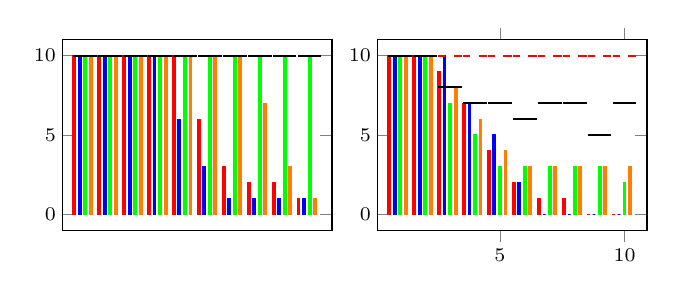
\begin{tikzpicture}
\tiny
    \begin{axis}[
    width =5cm,
    height=4cm,
    enlarge x limits = 0.1,
    enlarge y limits = 0.1,
    legend columns=1,
    ybar,
    bar width=1pt,
    ymin = 0,
    ymax = 10,
	compat=1.6,
	%title=c 100,
	%ylabel=goals 05,
	xticklabels={,,},
	xtick style={draw=none},
	at={(0,0)},
]
\addplot+[ybar, bar shift =-4.0pt, red,
]
plot coordinates {
(04, 10) %c_100
(05, 10) %c_100
(06, 6) %c_100
(01, 10) %c_100
(02, 10) %c_100
(08, 2) %c_100
(07, 3) %c_100
(03, 10) %c_100
(09, 2) %c_100
(10, 1) %c_100
};
\label{plot:props_bu_hff_94}
\addplot+[ybar, bar shift =-2.0pt, blue,
]
plot coordinates {
(04, 10) %c_100
(05, 6) %c_100
(06, 3) %c_100
(01, 10) %c_100
(02, 10) %c_100
(08, 1) %c_100
(07, 1) %c_100
(03, 10) %c_100
(09, 1) %c_100
(10, 1) %c_100
};
\label{plot:props_td_hff_94}
\addplot+[ybar, bar shift =0.0pt, green,
]
plot coordinates {
(04, 10) %c_100
(05, 10) %c_100
(06, 10) %c_100
(01, 10) %c_100
(02, 10) %c_100
(08, 10) %c_100
(10, 10) %c_100
(03, 10) %c_100
(09, 10) %c_100
(07, 10) %c_100
};
\label{plot:props_bu_trap_94}
\addplot+[ybar, bar shift =2.0pt, orange,
]
plot coordinates {
(04, 10) %c_100
(05, 10) %c_100
(06, 10) %c_100
(01, 10) %c_100
(02, 10) %c_100
(08, 7) %c_100
(07, 10) %c_100
(03, 10) %c_100
(09, 3) %c_100
(10, 1) %c_100
};
\label{plot:props_td_trap_94}

%lmcut
\addplot+[only marks, mark = -, mark options = {thick, red, dashed}, mark size = 0.15cm, black,
]
plot coordinates {
(01, 10)
(02, 10)
(03, 10)
(04, 10)
(05, 10)
(06, 10)
(07, 10)
(08, 10)
(09, 10)
(10, 10)
};

%trap first meta node top down
\addplot+[only marks, mark = -, mark options = {thick, black}, mark size = 0.15cm, black,
]
plot coordinates {
(01, 10)
(02, 10)
(03, 10)
(04, 10)
(05, 10)
(06, 10)
(07, 10)
(08, 10)
(09, 10)
(10, 10)
};

    \end{axis}
    \hfill
    
%\node[draw, align=center] (test) at (8,-18) {
%\ref{plot:props_bu_hff_94} props-bu-hff\\
%\ref{plot:props_td_hff_94} props-td-hff\\
%\ref{plot:props_bu_trap_94} props-bu-trap\\
%\ref{plot:props_td_trap_94} props-td-trap\\
%};

    \begin{axis}[
    width = 5cm,
    height=4cm,
    enlarge x limits = 0.1,
    enlarge y limits = 0.1,
    legend columns=1,
    ybar,
    bar width=1pt,
    ymin = 0,
    ymax = 10,
compat=1.6,
%title=c 150,
%ylabel=goals 6,
at={(4cm,0)},
]
\addplot+[ybar, bar shift =-4.0pt, red,
]
plot coordinates {
(08, 1) %c_150
(09, 0) %c_150
(03, 9) %c_150
(06, 2) %c_150
(07, 1) %c_150
(10, 0) %c_150
(04, 7) %c_150
(05, 4) %c_150
(01, 10) %c_150
(02, 10) %c_150
};
\label{plot:props_bu_hff_75}
\addplot+[ybar, bar shift =-2.0pt, blue,
]
plot coordinates {
(08, 0) %c_150
(09, 0) %c_150
(03, 10) %c_150
(06, 2) %c_150
(07, 0) %c_150
(10, 0) %c_150
(04, 7) %c_150
(05, 5) %c_150
(01, 10) %c_150
(02, 10) %c_150
};
\label{plot:props_td_hff_75}
\addplot+[ybar, bar shift =0.0pt, green,
]
plot coordinates {
(08, 3) %c_150
(09, 3) %c_150
(03, 7) %c_150
(06, 3) %c_150
(07, 3) %c_150
(10, 2) %c_150
(04, 5) %c_150
(05, 3) %c_150
(01, 10) %c_150
(02, 10) %c_150
};
\label{plot:props_bu_trap_75}
\addplot+[ybar, bar shift =2.0pt, orange,
]
plot coordinates {
(08, 3) %c_150
(09, 3) %c_150
(10, 3) %c_150
(06, 3) %c_150
(07, 3) %c_150
(03, 8) %c_150
(04, 6) %c_150
(05, 4) %c_150
(01, 10) %c_150
(02, 10) %c_150
};
\label{plot:props_td_trap_75}

%lmcut
\addplot+[only marks, mark = -, mark options = {thick, red, dashed}, mark size = 0.15cm, black,
]
plot coordinates {
(02, 10)
(01, 10)
(04, 10)
(03, 10)
(07, 10)
(08, 10)
(06, 10)
(10, 10)
(05, 10)
(09, 10)
};

%trap first meta node top down
\addplot+[only marks, mark = -, mark options = {thick, black}, mark size = 0.15cm, black,
]
plot coordinates {
(01, 10)
(02, 10)
(03, 8)
(04, 7)
(05, 7)
(06, 6)
(07, 7)
(08, 7)
(09, 5)
(10, 7)
};
    \end{axis}
    \hfill
    
%\node[draw, align=center] (test) at (8,-18) {
%\ref{plot:props_bu_hff_75} props-bu-hff\\
%\ref{plot:props_td_hff_75} props-td-hff\\
%\ref{plot:props_bu_trap_75} props-bu-trap\\
%\ref{plot:props_td_trap_75} props-td-trap\\
%%};



\end{tikzpicture}

\includegraphics{data/action_set_properties/barchart/barchart.pdf}
\vspace{-0.6cm}
\caption{Coverage results on IPC benchmarks extended with action-set properties.}
\label{fig:barcharts}
\vspace{-0.2cm}
\end{figure*}


\section{Experiments}
\label{experiments}

We implemented our approach in Fast Downward
(FD) \cite{helmert:jair-06}. We evaluate it, in turn, on IPC
benchmarks modified for oversubscription planning, and on a selection
of IPC benchmarks extended with action-set properties.

In all experiments, the base planner called by our SysS and SysW
algorithms on each search node
employs \hff\ \cite{hoffmann:nebel:jair-01} for search guidance.
%
%% The base planner configurations, used to solve/prove unsolvability
%% of a meta search node, are greedy best first search with $\hff$ and
%% preferred operators ($hff$) and conjunction learning $\hc$ with
%% $\hff$ as its base heuristic. \rebecca{ask Marcel how it is
%% called} \rebecca{Modification of hC to find deadends with an cost
%% bound}
%
The experiments were run on a cluster of Intel E5-2660 machines
running at 2.20 GHz, with time (memory) cut-offs of 30 minutes (4
GB).



 
\subsubsection*{Oversubscription Planning}

% The net-benefit benchmarks don't give us anything new (the ones we
% could use are adopted from IPC ben chmarks anyhow).
%
%% \joerg{Rebecca/Michael: check out the IPC net-benefit benchmarks. Reviewers may naturally expect us to experiment with those, given our strong focus on oversubscription planning (actually this question came up in the discussion with the NASA guys yesterday). In the net-bnefit benchmarks, goal facts have rewards which we don't need. The question is whether, stripping away these rewards and imposing a plan-cost bound, we would get benchmarks not already covered by bour IPC experiments anyway. If the answer is "no", we can just say so in the paper. If the answer is "yes", it would be good (though probably not absolitely necessary) to experiment with these domains as well. In any case, we should know what the answer is.}

To evaluate our analysis of goal dependencies in oversubscription
planning as per Section~\ref{goaldep}, we modified all
optimal-planning STRIPS IPC domains up to IPC'18. Following Domshlak
and Mirkis \shortcite{domshlak:mirkis:jair-15}, for each benchmark
task we ran an optimal planner (\astar
with \hlmcut\ \cite{helmert:domshlak:icaps-09}) to determine the
optimal plan cost $C$, then obtained OSP tasks by setting the cost
bound to $b = x * C$ where $x \in \{0.25, 0.5, 0.75\}$. Our benchmark
set consists of 46 domains, and contains those tasks solved by the
optimal planner, and where the number of goal facts is $\leq 32$.
%
%% ; the latter is an artifact of our current implementation that
%% could be overcome in principle, though computing all MUGS for that
%% many goals is presumably typically infeasible anyway.
%
We extended conjunction learning as per Steinmetz and
Hoffmann \shortcite{steinmetz:hoffmann:ai-17} to deal with cost
bounds, thus enabling nogood learning and transfer in SysS and
SysW. 

Figure~\ref{table:coverage_ipc} shows our data. Consider first the
coverage data (leftmost two parts). To have some sort of measure of
how computationally difficult our proposed analysis is, we use
reference points from classical planning. First, the \hlmcut\ column
gives coverage for \astar\ with \hlmcut\ run on the original IPC
instance without a cost bound. This provides a comparison to solvable
optimal planning. Second, the \hc\ columns give coverage for search
with nogood learning on the respective cost-bounded instances, when
all goals must be achieved and thus the task is unsolvable. This
provides a comparison to proving unsolvability in the situation where
our approach computes all MUGS. 
%
It is expected that our algorithms, solving a more complex problem,
will perform worse than the reference points.\footnote{Indeed, the
first reference point is an upper bound to our coverage, as only
solved instances are included in our benchmark set; and the second
reference point is an upper bound for SysW as it constitutes the first
search node in that algorithm.} The question is, how much worse? 

As a short summary of the answer provided by
Figure~\ref{table:coverage_ipc} to that question, compared to
the \hlmcut\ reference point, for $x=0.25$ the best of our four
configurations has equal coverage in 37 of the 46 domains, and in that
sense is ``not much'' worse than optimal planning. For larger cost
bounds, the solvable goal subsets become larger, and accordingly our
analysis becomes harder. For $x=0.5$ we get equal coverage in 23
domains, for $x=0.75$ in 15. The comparison to the \hc\
proving-unsolvability reference points is qualitatively similar, with
equal coverage in 38, 25, and 20 domains for $x=0.25, 0.5, 0.75$
respectively. Overall, it seems fair to say that our analyses can be
feasible in many cases (about half of the IPC domains), in the sense
of not being more infeasible than the most closely related classical
planning problems.

While comparing our algorithm configurations against each other is not
our focus here, observe in the rightmost part of
Figure~\ref{table:coverage_ipc} that both SysS and SysW suffer from
larger cost bounds, but that is less so for SysW. This is because, for
small cost bounds, solvable goal sets are small and thus SysS
terminates early; while for large cost bounds, solvable goal sets are
large and thus SysW terminates early. Conjunction learning (\hc\ in
the table) is moderately beneficial.
%
%% Comparing SysS and SysW, with cost bound 0.25 both show better
%% coverage in 4 domains. Among those domains, in \woodworking\
%% and \openstacks\ SysS explores a much smaller fraction of the
%% meta-search tree than SysW (0.02 vs. 0.99 and 0.06 vs. 0.99). With
%% a cost bound of 0.5 SysW has better coverage in more domains (8
%% vs. 6). With cost 0.75 both show better coverage in 7
%% domains. Although SysW explores the smaller fraction of the
%% meta-search tree, SysS still demonstrates better coverage
%% overall. \rebecca{In this setting, finding a plan is easier than
%% proving unsolvability?}
%
%% The table shows that $\hc$ is useful with SysW, but for SysS only
%% with cost bound is $0.25$.

Consider finally the \# MUGS part of
Figure~\ref{table:coverage_ipc}. Observe that, if the user asks a
question ``Why $r$ rather than $p$?'', the answer are the properties
entailed by $p$, represented here through the smallest conjunctions
excluded by $p$. The number of such conjunctions is at most the number
of MUGS. So \# MUGS corresponds to worst-case answer/explanation
size. As the data shows quite vividly, on average per domain that size
tends to be small, of a scale that seems feasible for human
inspection. (Taking the maximum rather than average per domain, the
average across domains is 31.8, 30.2, 13.3 for $x=0.25, 0.5, 0.75$
respectively.)

%
%% The average MUGS size for a cost bound of 0.25 is small (1.32). It
%% is often the case that for these problems, you cannot reach any of
%% the goal facts. In that case, the MUGS will be the goals.









\subsubsection*{Action Set Properties}

To evaluate the use of our framework with more complex plan
properties, beyond goal facts, we experimented with the compilation of
action-set properties as per Section~\ref{compilation}. We selected
four IPC domains for extension with action-set properties, namely
NoMystery, Rovers, and TPP as considered in resource-constrained
planning \cite{nakhost:etal:icaps-12}, where optimal resource
requirements can be controlled through available problem generators;
plus the Blocksworld as an intuitively rather differently structured
domain. In all four domains, we use discrete resource consumption
encoded into the STRIPS model. We set the available resources to
$x \in \{1.0,1.5, 2.0\}$ times the minimum needed, and we chose the
size parameters in a way targetting the borderline of computational
feasibility given our time/memory limits. We vary the number of hard
goals between 4 and 7, and the number of action set properties between
1 and 10. In NoMystery, the action-set properties are as in the
illustrative example given in Section~\ref{illustrative-example}. In
Blocksworld, we include two gripper hands and the action-set
properties ask whether a particular gripper is used to pick up a
particular block, or to stack a particular pair of blocks. In Rovers,
the properties ask whether a particular rover or camera is used for a
particular observation. In TPP, they ask whether particular road
segments are used, and whether particular goods are bought at
particular markets.

%% \begin{enumerate}
%% \item The resource constrained \textit{rovers} domain. Problems were generated with 2 rovers, 5 waypoints. Action properties are to use a specific rover for a sample or an observation, or to use a specific camera for an observation. 
%% \item The \textit{blocksworld} domain with 2 grippers, modified such that picking up or unstacking a block costs high or low energy depending upon which gripper is used. Problems were generated scaling from 3 to 10 blocks. Action properties are to use a specific gripper to pick up a specific block, or to use any gripper to stack a specific pair of blocks at any point in the plan.
%% \item The resource constrained \textit{TPP} domain. Problems were generated with 5 markets and 1 depot. Properties are to use or not use particular road segments, and preferred markets for goods.
%% \item The resource constrained \textit{nomystery} domain, described in the example. Problems were generated with 6 locations and 2 trucks.
%% \end{enumerate}

Figure~\ref{fig:barcharts} shows coverage data, comparing against the
same reference points as before. For space reasons, we show only one
row per domain, fixing the number of hard goals at the feasibility
borderline (smaller numbers of hard goals tend to be quite easy,
larger ones largely infeasible, with variance depending on the domain
etc). Our algorithm configurations here are SysS and SysW as before,
now with vs.\ without trap learning (which can deal only with STRIPS,
not with the cost bounds used in oversubscription planning
above). Similarly as for Figure~\ref{table:coverage_ipc}, the data
shows that our analyses can be feasible compared to the reference
points; although that depends, of course, on the domain and on
instance size. Trap learning and transfer turns out to be extremely
useful here, vastly outperforming the non-learning algorithm in many
cases.

%\begin{figure*}[ht]
%
\tiny
\begin{tikzpicture}


\begin{axis}[
width = 7cm,
height=4cm,
enlarge x limits = 0.1,
enlarge y limits = 0.1,
ybar,
bar width=1pt,
ymin = 0,
ymax = 10,
at={(0.0\linewidth,-0.0)},
compat=1.6,
title=c 100,
ylabel=goals 4,
]
\addplot+[ybar, bar shift =-2.5pt, red,
]
plot coordinates {
(07, 10)
(08, 10)
(01, 10)
(09, 10)
(06, 10)
(03, 10)
(04, 10)
(05, 10)
(02, 10)
(10, 9)
};
\label{plot:properties_hff_bu_55}
\addplot+[ybar, bar shift =-0.5pt, blue,
]
plot coordinates {
(08, 10)
(01, 10)
(07, 10)
(09, 9)
(06, 10)
(03, 10)
(04, 10)
(05, 10)
(02, 10)
(10, 9)
};
\label{plot:properties_hff_td_55}
\addplot+[ybar, bar shift =0.5pt, darkgreen,
]
plot coordinates {
(05, 10)
(08, 10)
(07, 10)
(09, 10)
(03, 10)
(04, 10)
(06, 10)
(01, 10)
(10, 10)
(02, 10)
};
\label{plot:properties_trap_prefop_bu_55}
\addplot+[ybar, bar shift =2.5pt, orange,
]
plot coordinates {
(07, 10)
(05, 10)
(04, 10)
(08, 10)
(09, 10)
(03, 10)
(06, 10)
(01, 10)
(10, 10)
(02, 10)
};
\label{plot:properties_trap_prefop_td_55}

\end{axis}
\hfill


\begin{axis}[
width = 7cm,
height=4cm,
enlarge x limits = 0.1,
enlarge y limits = 0.1,
ybar,
bar width=1pt,
ymin = 0,
ymax = 10,
at={(0.333333333333\linewidth,-0.0)},
compat=1.6,
title=c 150,
]
\addplot+[ybar, bar shift =-2.5pt, red,
]
plot coordinates {
(05, 9)
(04, 10)
(03, 10)
(10, 1)
(02, 10)
(06, 8)
(09, 1)
(08, 2)
(07, 5)
(01, 10)
};
\label{plot:properties_hff_bu_55}
\addplot+[ybar, bar shift =-0.5pt, blue,
]
plot coordinates {
(05, 9)
(04, 10)
(10, 0)
(02, 10)
(09, 0)
(08, 2)
(03, 10)
(07, 3)
(06, 7)
(01, 10)
};
\label{plot:properties_hff_td_55}
\addplot+[ybar, bar shift =0.5pt, darkgreen,
]
plot coordinates {
(05, 8)
(04, 9)
(10, 2)
(02, 10)
(09, 2)
(08, 3)
(03, 10)
(07, 5)
(06, 6)
(01, 10)
};
\label{plot:properties_trap_prefop_bu_55}
\addplot+[ybar, bar shift =2.5pt, orange,
]
plot coordinates {
(05, 10)
(04, 10)
(10, 2)
(02, 10)
(08, 4)
(03, 10)
(07, 6)
(06, 9)
(01, 10)
(09, 3)
};
\label{plot:properties_trap_prefop_td_55}

\end{axis}
\hfill


\begin{axis}[
width = 7cm,
height=4cm,
enlarge x limits = 0.1,
enlarge y limits = 0.1,
ybar,
bar width=1pt,
ymin = 0,
ymax = 10,
at={(0.666666666667\linewidth,-0.0)},
compat=1.6,
title=c 200,
]
\addplot+[ybar, bar shift =-2.5pt, red,
]
plot coordinates {
(08, 1)
(02, 10)
(03, 10)
(04, 10)
(07, 2)
(09, 0)
(01, 10)
(06, 6)
(10, 0)
(05, 10)
};
\label{plot:properties_hff_bu_55}
\addplot+[ybar, bar shift =-0.5pt, blue,
]
plot coordinates {
(07, 8)
(08, 6)
(02, 10)
(03, 10)
(04, 10)
(09, 5)
(10, 2)
(01, 10)
(06, 9)
(05, 10)
};
\label{plot:properties_hff_td_55}
\addplot+[ybar, bar shift =0.5pt, darkgreen,
]
plot coordinates {
(08, 2)
(07, 3)
(03, 10)
(06, 5)
(04, 10)
(09, 0)
(01, 10)
(02, 10)
(05, 9)
(10, 0)
};
\label{plot:properties_trap_prefop_bu_55}
\addplot+[ybar, bar shift =2.5pt, orange,
]
plot coordinates {
(08, 9)
(07, 8)
(06, 10)
(04, 10)
(01, 10)
(10, 5)
(03, 10)
(09, 8)
(02, 10)
(05, 10)
};
\label{plot:properties_trap_prefop_td_55}

\end{axis}
\hfill


\begin{axis}[
width = 7cm,
height=4cm,
enlarge x limits = 0.1,
enlarge y limits = 0.1,
ybar,
bar width=1pt,
ymin = 0,
ymax = 10,
at={(0.0\linewidth,-160.0)},
compat=1.6,
ylabel=goals 5,
]
\addplot+[ybar, bar shift =-2.5pt, red,
]
plot coordinates {
(01, 10)
(08, 9)
(05, 10)
(03, 10)
(02, 10)
(09, 9)
(04, 10)
(07, 9)
(06, 10)
(10, 9)
};
\label{plot:properties_hff_bu_55}
\addplot+[ybar, bar shift =-0.5pt, blue,
]
plot coordinates {
(01, 10)
(08, 6)
(03, 10)
(02, 10)
(09, 5)
(04, 10)
(07, 7)
(05, 10)
(06, 9)
(10, 2)
};
\label{plot:properties_hff_td_55}
\addplot+[ybar, bar shift =0.5pt, darkgreen,
]
plot coordinates {
(01, 10)
(08, 10)
(03, 10)
(02, 10)
(07, 10)
(05, 10)
(04, 10)
(09, 10)
(06, 10)
(10, 10)
};
\label{plot:properties_trap_prefop_bu_55}
\addplot+[ybar, bar shift =2.5pt, orange,
]
plot coordinates {
(01, 10)
(08, 10)
(03, 10)
(02, 10)
(09, 10)
(07, 10)
(04, 10)
(06, 10)
(10, 10)
(05, 10)
};
\label{plot:properties_trap_prefop_td_55}

\end{axis}
\hfill


\begin{axis}[
width = 7cm,
height=4cm,
enlarge x limits = 0.1,
enlarge y limits = 0.1,
ybar,
bar width=1pt,
ymin = 0,
ymax = 10,
at={(0.333333333333\linewidth,-160.0)},
compat=1.6,
]
\addplot+[ybar, bar shift =-2.5pt, red,
]
plot coordinates {
(05, 5)
(06, 2)
(10, 0)
(04, 9)
(01, 10)
(09, 0)
(02, 10)
(08, 1)
(07, 1)
(03, 10)
};
\label{plot:properties_hff_bu_55}
\addplot+[ybar, bar shift =-0.5pt, blue,
]
plot coordinates {
(05, 7)
(06, 4)
(10, 1)
(04, 9)
(01, 10)
(09, 1)
(02, 10)
(08, 1)
(07, 1)
(03, 10)
};
\label{plot:properties_hff_td_55}
\addplot+[ybar, bar shift =0.5pt, darkgreen,
]
plot coordinates {
(05, 6)
(06, 2)
(10, 1)
(04, 10)
(01, 10)
(09, 1)
(02, 10)
(08, 1)
(07, 1)
(03, 10)
};
\label{plot:properties_trap_prefop_bu_55}
\addplot+[ybar, bar shift =2.5pt, orange,
]
plot coordinates {
(05, 9)
(06, 6)
(10, 2)
(04, 10)
(01, 10)
(09, 2)
(02, 10)
(08, 3)
(07, 4)
(03, 10)
};
\label{plot:properties_trap_prefop_td_55}

\end{axis}
\hfill


\begin{axis}[
width = 7cm,
height=4cm,
enlarge x limits = 0.1,
enlarge y limits = 0.1,
ybar,
bar width=1pt,
ymin = 0,
ymax = 10,
at={(0.666666666667\linewidth,-160.0)},
compat=1.6,
]
\addplot+[ybar, bar shift =-2.5pt, red,
]
plot coordinates {
(03, 10)
(04, 7)
(05, 3)
(09, 0)
(01, 10)
(02, 10)
(08, 0)
(06, 1)
(10, 0)
(07, 0)
};
\label{plot:properties_hff_bu_55}
\addplot+[ybar, bar shift =-0.5pt, blue,
]
plot coordinates {
(03, 10)
(04, 8)
(05, 7)
(09, 5)
(01, 10)
(02, 10)
(08, 5)
(06, 7)
(10, 4)
(07, 6)
};
\label{plot:properties_hff_td_55}
\addplot+[ybar, bar shift =0.5pt, darkgreen,
]
plot coordinates {
(03, 9)
(04, 6)
(05, 1)
(09, 0)
(01, 10)
(02, 10)
(08, 0)
(06, 1)
(10, 0)
(07, 0)
};
\label{plot:properties_trap_prefop_bu_55}
\addplot+[ybar, bar shift =2.5pt, orange,
]
plot coordinates {
(03, 10)
(04, 10)
(05, 8)
(09, 5)
(01, 10)
(02, 10)
(08, 6)
(07, 8)
(06, 7)
(10, 4)
};
\label{plot:properties_trap_prefop_td_55}

\end{axis}
\hfill


\begin{axis}[
width = 7cm,
height=4cm,
enlarge x limits = 0.1,
enlarge y limits = 0.1,
ybar,
bar width=1pt,
ymin = 0,
ymax = 10,
at={(0.0\linewidth,-320.0)},
compat=1.6,
ylabel=goals 6,
]
\addplot+[ybar, bar shift =-2.5pt, red,
]
plot coordinates {
(08, 2)
(09, 2)
(01, 10)
(10, 2)
(06, 5)
(04, 8)
(07, 4)
(05, 5)
(02, 9)
(03, 8)
};
\label{plot:properties_hff_bu_55}
\addplot+[ybar, bar shift =-0.5pt, blue,
]
plot coordinates {
(06, 2)
(08, 2)
(09, 2)
(01, 10)
(10, 2)
(07, 2)
(04, 7)
(05, 4)
(02, 9)
(03, 8)
};
\label{plot:properties_hff_td_55}
\addplot+[ybar, bar shift =0.5pt, darkgreen,
]
plot coordinates {
(08, 8)
(09, 8)
(01, 10)
(10, 8)
(06, 9)
(04, 10)
(02, 10)
(05, 9)
(07, 8)
(03, 10)
};
\label{plot:properties_trap_prefop_bu_55}
\addplot+[ybar, bar shift =2.5pt, orange,
]
plot coordinates {
(08, 8)
(09, 8)
(01, 10)
(10, 7)
(06, 7)
(04, 8)
(07, 8)
(05, 7)
(03, 8)
(02, 10)
};
\label{plot:properties_trap_prefop_td_55}

\end{axis}
\hfill


\begin{axis}[
width = 7cm,
height=4cm,
enlarge x limits = 0.1,
enlarge y limits = 0.1,
ybar,
bar width=1pt,
ymin = 0,
ymax = 10,
at={(0.333333333333\linewidth,-320.0)},
compat=1.6,
]
\addplot+[ybar, bar shift =-2.5pt, red,
]
plot coordinates {
(06, 1)
(10, 0)
(03, 9)
(05, 3)
(07, 1)
(08, 1)
(02, 10)
(09, 0)
(01, 10)
(04, 7)
};
\label{plot:properties_hff_bu_55}
\addplot+[ybar, bar shift =-0.5pt, blue,
]
plot coordinates {
(06, 2)
(10, 0)
(03, 10)
(05, 4)
(08, 0)
(07, 0)
(02, 10)
(09, 0)
(01, 10)
(04, 7)
};
\label{plot:properties_hff_td_55}
\addplot+[ybar, bar shift =0.5pt, darkgreen,
]
plot coordinates {
(06, 2)
(10, 2)
(05, 2)
(08, 2)
(07, 2)
(02, 10)
(09, 2)
(01, 10)
(03, 7)
(04, 4)
};
\label{plot:properties_trap_prefop_bu_55}
\addplot+[ybar, bar shift =2.5pt, orange,
]
plot coordinates {
(06, 3)
(10, 3)
(03, 8)
(05, 4)
(07, 3)
(08, 3)
(02, 10)
(09, 3)
(01, 10)
(04, 6)
};
\label{plot:properties_trap_prefop_td_55}

\end{axis}
\hfill


\begin{axis}[
width = 7cm,
height=4cm,
enlarge x limits = 0.1,
enlarge y limits = 0.1,
ybar,
bar width=1pt,
ymin = 0,
ymax = 10,
at={(0.666666666667\linewidth,-320.0)},
compat=1.6,
]
\addplot+[ybar, bar shift =-2.5pt, red,
]
plot coordinates {
(02, 8)
(01, 10)
(04, 3)
(03, 4)
(06, 1)
(10, 0)
(05, 3)
(09, 0)
(08, 0)
(07, 0)
};
\label{plot:properties_hff_bu_55}
\addplot+[ybar, bar shift =-0.5pt, blue,
]
plot coordinates {
(02, 9)
(01, 10)
(04, 6)
(03, 7)
(08, 3)
(06, 4)
(10, 1)
(05, 6)
(09, 1)
(07, 4)
};
\label{plot:properties_hff_td_55}
\addplot+[ybar, bar shift =0.5pt, darkgreen,
]
plot coordinates {
(02, 10)
(01, 10)
(06, 1)
(04, 4)
(03, 5)
(08, 0)
(10, 0)
(05, 2)
(09, 0)
(07, 0)
};
\label{plot:properties_trap_prefop_bu_55}
\addplot+[ybar, bar shift =2.5pt, orange,
]
plot coordinates {
(02, 10)
(04, 7)
(03, 8)
(07, 5)
(08, 4)
(06, 7)
(10, 3)
(05, 7)
(09, 3)
(01, 10)
};
\label{plot:properties_trap_prefop_td_55}

\end{axis}
\hfill

\node[draw] (test) at (8,-8) {
\ref{plot:properties_hff_bu_55} properties-hff-bu
\ref{plot:properties_hff_td_55} properties-hff-td
\ref{plot:properties_trap_prefop_bu_55} properties-trap-prefop-bu
\ref{plot:properties_trap_prefop_td_55} properties-trap-prefop-td
};

\end{tikzpicture}
\hfill

%\caption{nomystery: reference coverage first node in top-down meta search tree;
%	optimal coverage always 10}
%\end{figure*}

%\begin{figure*}[ht]
%
\tiny
\begin{tikzpicture}


\begin{axis}[
width = 7cm,
height=4cm,
enlarge x limits = 0.1,
enlarge y limits = 0.1,
ybar,
bar width=1pt,
ymin = 0,
ymax = 10,
at={(0.0\linewidth,-0.0)},
compat=1.6,
title=c 100,
ylabel=goals 4,
]
\addplot+[ybar, bar shift =-2.5pt, red,
]
plot coordinates {
(04, 10)
(03, 10)
(02, 10)
(09, 10)
(01, 10)
(08, 10)
(07, 10)
(10, 10)
(06, 10)
(05, 10)
};
\label{plot:properties_hff_bu_4}
\addplot+[ybar, bar shift =-0.5pt, blue,
]
plot coordinates {
(04, 10)
(03, 10)
(02, 10)
(09, 10)
(01, 10)
(08, 10)
(07, 10)
(10, 10)
(06, 10)
(05, 10)
};
\label{plot:properties_hff_td_4}
\addplot+[ybar, bar shift =0.5pt, darkgreen,
]
plot coordinates {
(04, 10)
(03, 10)
(02, 10)
(09, 10)
(01, 10)
(08, 10)
(07, 10)
(10, 10)
(06, 10)
(05, 10)
};
\label{plot:properties_trap_prefop_bu_4}
\addplot+[ybar, bar shift =2.5pt, orange,
]
plot coordinates {
(04, 10)
(03, 10)
(02, 10)
(09, 10)
(01, 10)
(08, 10)
(07, 10)
(10, 10)
(06, 10)
(05, 10)
};
\label{plot:properties_trap_prefop_td_4}

\end{axis}
\hfill


\begin{axis}[
width = 7cm,
height=4cm,
enlarge x limits = 0.1,
enlarge y limits = 0.1,
ybar,
bar width=1pt,
ymin = 0,
ymax = 10,
at={(0.333333333333\linewidth,-0.0)},
compat=1.6,
title=c 150,
]
\addplot+[ybar, bar shift =-2.5pt, red,
]
plot coordinates {
(07, 10)
(08, 10)
(09, 10)
(01, 10)
(02, 10)
(03, 10)
(04, 10)
(05, 10)
(06, 10)
(10, 10)
};
\label{plot:properties_hff_bu_4}
\addplot+[ybar, bar shift =-0.5pt, blue,
]
plot coordinates {
(07, 10)
(08, 10)
(09, 8)
(01, 10)
(04, 10)
(02, 10)
(03, 10)
(05, 10)
(10, 4)
(06, 10)
};
\label{plot:properties_hff_td_4}
\addplot+[ybar, bar shift =0.5pt, darkgreen,
]
plot coordinates {
(07, 10)
(08, 9)
(09, 9)
(01, 10)
(02, 10)
(03, 10)
(04, 10)
(05, 10)
(06, 10)
(10, 9)
};
\label{plot:properties_trap_prefop_bu_4}
\addplot+[ybar, bar shift =2.5pt, orange,
]
plot coordinates {
(07, 10)
(08, 10)
(09, 10)
(01, 10)
(02, 10)
(03, 10)
(04, 10)
(05, 10)
(06, 10)
(10, 10)
};
\label{plot:properties_trap_prefop_td_4}

\end{axis}
\hfill


\begin{axis}[
width = 7cm,
height=4cm,
enlarge x limits = 0.1,
enlarge y limits = 0.1,
ybar,
bar width=1pt,
ymin = 0,
ymax = 10,
at={(0.666666666667\linewidth,-0.0)},
compat=1.6,
title=c 200,
]
\addplot+[ybar, bar shift =-2.5pt, red,
]
plot coordinates {
(07, 10)
(04, 10)
(05, 10)
(06, 10)
(10, 9)
(03, 10)
(08, 10)
(01, 10)
(09, 10)
(02, 10)
};
\label{plot:properties_hff_bu_4}
\addplot+[ybar, bar shift =-0.5pt, blue,
]
plot coordinates {
(05, 10)
(04, 10)
(06, 10)
(10, 8)
(07, 10)
(03, 10)
(08, 10)
(01, 10)
(09, 8)
(02, 10)
};
\label{plot:properties_hff_td_4}
\addplot+[ybar, bar shift =0.5pt, darkgreen,
]
plot coordinates {
(08, 10)
(03, 10)
(05, 10)
(04, 10)
(10, 8)
(02, 10)
(07, 10)
(01, 10)
(09, 9)
(06, 10)
};
\label{plot:properties_trap_prefop_bu_4}
\addplot+[ybar, bar shift =2.5pt, orange,
]
plot coordinates {
(05, 10)
(04, 10)
(10, 10)
(07, 10)
(03, 10)
(08, 10)
(01, 10)
(09, 10)
(06, 10)
(02, 10)
};
\label{plot:properties_trap_prefop_td_4}

\end{axis}
\hfill


\begin{axis}[
width = 7cm,
height=4cm,
enlarge x limits = 0.1,
enlarge y limits = 0.1,
ybar,
bar width=1pt,
ymin = 0,
ymax = 10,
at={(0.0\linewidth,-160.0)},
compat=1.6,
ylabel=goals 5,
]
\addplot+[ybar, bar shift =-2.5pt, red,
]
plot coordinates {
(08, 10)
(04, 10)
(09, 10)
(01, 10)
(06, 10)
(07, 10)
(02, 10)
(03, 10)
(05, 10)
(10, 10)
};
\label{plot:properties_hff_bu_4}
\addplot+[ybar, bar shift =-0.5pt, blue,
]
plot coordinates {
(03, 10)
(08, 9)
(01, 10)
(09, 7)
(07, 10)
(02, 10)
(04, 10)
(06, 10)
(05, 10)
(10, 4)
};
\label{plot:properties_hff_td_4}
\addplot+[ybar, bar shift =0.5pt, darkgreen,
]
plot coordinates {
(03, 10)
(08, 10)
(01, 10)
(09, 10)
(07, 10)
(04, 10)
(06, 10)
(05, 10)
(10, 10)
(02, 10)
};
\label{plot:properties_trap_prefop_bu_4}
\addplot+[ybar, bar shift =2.5pt, orange,
]
plot coordinates {
(08, 10)
(03, 10)
(09, 10)
(01, 10)
(06, 10)
(07, 10)
(04, 10)
(05, 10)
(10, 10)
(02, 10)
};
\label{plot:properties_trap_prefop_td_4}

\end{axis}
\hfill


\begin{axis}[
width = 7cm,
height=4cm,
enlarge x limits = 0.1,
enlarge y limits = 0.1,
ybar,
bar width=1pt,
ymin = 0,
ymax = 10,
at={(0.333333333333\linewidth,-160.0)},
compat=1.6,
]
\addplot+[ybar, bar shift =-2.5pt, red,
]
plot coordinates {
(02, 10)
(05, 10)
(10, 3)
(04, 10)
(07, 7)
(06, 9)
(09, 3)
(01, 10)
(08, 6)
(03, 10)
};
\label{plot:properties_hff_bu_4}
\addplot+[ybar, bar shift =-0.5pt, blue,
]
plot coordinates {
(02, 10)
(10, 2)
(05, 10)
(04, 10)
(07, 7)
(06, 9)
(09, 2)
(01, 10)
(08, 5)
(03, 10)
};
\label{plot:properties_hff_td_4}
\addplot+[ybar, bar shift =0.5pt, darkgreen,
]
plot coordinates {
(02, 10)
(10, 5)
(05, 10)
(04, 10)
(07, 9)
(06, 10)
(09, 8)
(01, 10)
(08, 8)
(03, 10)
};
\label{plot:properties_trap_prefop_bu_4}
\addplot+[ybar, bar shift =2.5pt, orange,
]
plot coordinates {
(02, 10)
(10, 7)
(04, 10)
(05, 10)
(07, 10)
(06, 10)
(09, 10)
(01, 10)
(08, 10)
(03, 10)
};
\label{plot:properties_trap_prefop_td_4}

\end{axis}
\hfill


\begin{axis}[
width = 7cm,
height=4cm,
enlarge x limits = 0.1,
enlarge y limits = 0.1,
ybar,
bar width=1pt,
ymin = 0,
ymax = 10,
at={(0.666666666667\linewidth,-160.0)},
compat=1.6,
]
\addplot+[ybar, bar shift =-2.5pt, red,
]
plot coordinates {
(02, 10)
(05, 10)
(04, 10)
(07, 9)
(06, 10)
(10, 8)
(03, 10)
(09, 9)
(01, 10)
(08, 9)
};
\label{plot:properties_hff_bu_4}
\addplot+[ybar, bar shift =-0.5pt, blue,
]
plot coordinates {
(03, 10)
(02, 10)
(10, 8)
(05, 10)
(04, 10)
(07, 9)
(06, 10)
(09, 9)
(01, 10)
(08, 9)
};
\label{plot:properties_hff_td_4}
\addplot+[ybar, bar shift =0.5pt, darkgreen,
]
plot coordinates {
(07, 9)
(03, 10)
(02, 10)
(10, 6)
(05, 10)
(04, 10)
(06, 10)
(09, 7)
(01, 10)
(08, 8)
};
\label{plot:properties_trap_prefop_bu_4}
\addplot+[ybar, bar shift =2.5pt, orange,
]
plot coordinates {
(03, 10)
(02, 10)
(10, 9)
(05, 10)
(04, 10)
(07, 10)
(06, 10)
(09, 10)
(01, 10)
(08, 10)
};
\label{plot:properties_trap_prefop_td_4}

\end{axis}
\hfill


\begin{axis}[
width = 7cm,
height=4cm,
enlarge x limits = 0.1,
enlarge y limits = 0.1,
ybar,
bar width=1pt,
ymin = 0,
ymax = 10,
at={(0.0\linewidth,-320.0)},
compat=1.6,
ylabel=goals 6,
]
\addplot+[ybar, bar shift =-2.5pt, red,
]
plot coordinates {
(10, 7)
(09, 8)
(02, 10)
(05, 10)
(03, 10)
(06, 10)
(01, 10)
(08, 9)
(07, 9)
(04, 10)
};
\label{plot:properties_hff_bu_4}
\addplot+[ybar, bar shift =-0.5pt, blue,
]
plot coordinates {
(09, 0)
(02, 10)
(07, 4)
(05, 9)
(03, 10)
(04, 10)
(10, 0)
(01, 10)
(08, 1)
(06, 8)
};
\label{plot:properties_hff_td_4}
\addplot+[ybar, bar shift =0.5pt, darkgreen,
]
plot coordinates {
(10, 10)
(04, 10)
(05, 10)
(07, 10)
(06, 10)
(01, 10)
(02, 10)
(09, 10)
(08, 10)
(03, 10)
};
\label{plot:properties_trap_prefop_bu_4}
\addplot+[ybar, bar shift =2.5pt, orange,
]
plot coordinates {
(10, 10)
(09, 10)
(02, 10)
(05, 10)
(04, 10)
(03, 10)
(07, 10)
(01, 10)
(08, 10)
(06, 10)
};
\label{plot:properties_trap_prefop_td_4}

\end{axis}
\hfill


\begin{axis}[
width = 7cm,
height=4cm,
enlarge x limits = 0.1,
enlarge y limits = 0.1,
ybar,
bar width=1pt,
ymin = 0,
ymax = 10,
at={(0.333333333333\linewidth,-320.0)},
compat=1.6,
]
\addplot+[ybar, bar shift =-2.5pt, red,
]
plot coordinates {
(10, 2)
(02, 10)
(03, 10)
(08, 3)
(01, 10)
(06, 5)
(07, 3)
(09, 2)
(04, 9)
(05, 8)
};
\label{plot:properties_hff_bu_4}
\addplot+[ybar, bar shift =-0.5pt, blue,
]
plot coordinates {
(10, 3)
(02, 10)
(03, 10)
(08, 3)
(01, 10)
(06, 5)
(07, 3)
(09, 3)
(04, 9)
(05, 8)
};
\label{plot:properties_hff_td_4}
\addplot+[ybar, bar shift =0.5pt, darkgreen,
]
plot coordinates {
(10, 4)
(02, 10)
(03, 10)
(08, 6)
(01, 10)
(09, 5)
(06, 10)
(07, 7)
(04, 10)
(05, 10)
};
\label{plot:properties_trap_prefop_bu_4}
\addplot+[ybar, bar shift =2.5pt, orange,
]
plot coordinates {
(10, 5)
(02, 10)
(03, 10)
(08, 8)
(01, 10)
(06, 10)
(07, 9)
(09, 6)
(04, 10)
(05, 10)
};
\label{plot:properties_trap_prefop_td_4}

\end{axis}
\hfill


\begin{axis}[
width = 7cm,
height=4cm,
enlarge x limits = 0.1,
enlarge y limits = 0.1,
ybar,
bar width=1pt,
ymin = 0,
ymax = 10,
at={(0.666666666667\linewidth,-320.0)},
compat=1.6,
]
\addplot+[ybar, bar shift =-2.5pt, red,
]
plot coordinates {
(04, 10)
(05, 10)
(02, 10)
(03, 10)
(06, 9)
(08, 8)
(09, 8)
(01, 10)
(07, 8)
(10, 7)
};
\label{plot:properties_hff_bu_4}
\addplot+[ybar, bar shift =-0.5pt, blue,
]
plot coordinates {
(04, 10)
(05, 10)
(02, 10)
(03, 10)
(06, 9)
(08, 8)
(09, 8)
(01, 10)
(07, 9)
(10, 7)
};
\label{plot:properties_hff_td_4}
\addplot+[ybar, bar shift =0.5pt, darkgreen,
]
plot coordinates {
(04, 10)
(05, 10)
(02, 10)
(03, 10)
(08, 6)
(09, 4)
(01, 10)
(06, 10)
(07, 7)
(10, 3)
};
\label{plot:properties_trap_prefop_bu_4}
\addplot+[ybar, bar shift =2.5pt, orange,
]
plot coordinates {
(04, 10)
(05, 10)
(02, 10)
(03, 10)
(08, 10)
(09, 9)
(01, 10)
(06, 10)
(07, 10)
(10, 8)
};
\label{plot:properties_trap_prefop_td_4}

\end{axis}
\hfill

\node[draw] (test) at (8,-8) {
\ref{plot:properties_hff_bu_4} properties-hff-bu
\ref{plot:properties_hff_td_4} properties-hff-td
\ref{plot:properties_trap_prefop_bu_4} properties-trap-prefop-bu
\ref{plot:properties_trap_prefop_td_4} properties-trap-prefop-td
};

\end{tikzpicture}
\hfill

%\caption{TPP: reference coverage first node in top-down meta search tree;
%	optimal coverage always 10}
%\end{figure*}

%\begin{figure*}[ht]
%
\tiny
\begin{tikzpicture}


\begin{axis}[
width = 7cm,
height=4cm,
enlarge x limits = 0.1,
enlarge y limits = 0.1,
ybar,
bar width=1pt,
ymin = 0,
ymax = 10,
at={(0.0\linewidth,-0.0)},
compat=1.6,
title=c 100,
ylabel=goals 05,
]
\addplot+[ybar, bar shift =-2.5pt, red,
]
plot coordinates {
(05, 10)
(04, 10)
(06, 9)
(02, 10)
(10, 6)
(01, 10)
(08, 9)
(09, 7)
(03, 10)
(07, 8)
};
\label{plot:properties_hff_bu_52}
\addplot+[ybar, bar shift =-1.0pt, blue,
]
plot coordinates {
(06, 9)
(10, 4)
(05, 10)
(04, 10)
(02, 10)
(01, 10)
(08, 5)
(09, 5)
(07, 7)
(03, 10)
};
\label{plot:properties_hff_td_52}
\addplot+[ybar, bar shift =1.0pt, darkgreen,
]
plot coordinates {
(06, 10)
(10, 10)
(05, 10)
(04, 10)
(03, 10)
(02, 10)
(01, 10)
(08, 10)
(09, 10)
(07, 10)
};
\label{plot:properties_trap_prefop_bu_52}
\addplot+[ybar, bar shift =2.5pt, orange,
]
plot coordinates {
(06, 10)
(05, 10)
(03, 10)
(07, 10)
(10, 10)
(02, 10)
(01, 10)
(08, 10)
(09, 10)
(04, 10)
};
\label{plot:properties_trap_prefop_td_52}
\addplot+[only marks, mark = -, mark options = {thick, red, dashed}, mark size = 0.2cm, black,
]
plot coordinates {
(08, 6)
(06, 6)
(05, 8)
(03, 9)
(01, 10)
(09, 6)
(07, 4)
(10, 4)
(04, 8)
(02, 10)
};

\end{axis}
\hfill


\begin{axis}[
width = 7cm,
height=4cm,
enlarge x limits = 0.1,
enlarge y limits = 0.1,
ybar,
bar width=1pt,
ymin = 0,
ymax = 10,
at={(0.333333333333\linewidth,-0.0)},
compat=1.6,
title=c 150,
]
\addplot+[ybar, bar shift =-2.5pt, red,
]
plot coordinates {
(08, 5)
(01, 10)
(09, 5)
(06, 8)
(07, 5)
(04, 9)
(05, 10)
(10, 4)
(02, 10)
(03, 9)
};
\label{plot:properties_hff_bu_52}
\addplot+[ybar, bar shift =-1.0pt, blue,
]
plot coordinates {
(01, 10)
(08, 4)
(09, 4)
(06, 4)
(07, 4)
(04, 9)
(05, 9)
(10, 4)
(02, 10)
(03, 9)
};
\label{plot:properties_hff_td_52}
\addplot+[ybar, bar shift =1.0pt, darkgreen,
]
plot coordinates {
(08, 10)
(01, 10)
(09, 10)
(06, 10)
(07, 10)
(04, 10)
(05, 10)
(10, 10)
(02, 10)
(03, 10)
};
\label{plot:properties_trap_prefop_bu_52}
\addplot+[ybar, bar shift =2.5pt, orange,
]
plot coordinates {
(08, 10)
(01, 10)
(09, 10)
(06, 10)
(07, 10)
(04, 10)
(05, 10)
(10, 10)
(02, 10)
(03, 10)
};
\label{plot:properties_trap_prefop_td_52}
\addplot+[only marks, mark = -, mark options = {thick, red, dashed}, mark size = 0.2cm, black,
]
plot coordinates {
(08, 6)
(06, 6)
(05, 8)
(03, 9)
(01, 10)
(09, 6)
(07, 4)
(10, 4)
(04, 8)
(02, 10)
};

\end{axis}
\hfill


\begin{axis}[
width = 7cm,
height=4cm,
enlarge x limits = 0.1,
enlarge y limits = 0.1,
ybar,
bar width=1pt,
ymin = 0,
ymax = 10,
at={(0.666666666667\linewidth,-0.0)},
compat=1.6,
title=c 200,
]
\addplot+[ybar, bar shift =-2.5pt, red,
]
plot coordinates {
(08, 8)
(04, 10)
(05, 10)
(10, 6)
(02, 10)
(03, 10)
(09, 9)
(01, 10)
(06, 7)
(07, 6)
};
\label{plot:properties_hff_bu_52}
\addplot+[ybar, bar shift =-1.0pt, blue,
]
plot coordinates {
(04, 10)
(05, 10)
(10, 7)
(02, 10)
(03, 10)
(08, 8)
(09, 9)
(01, 10)
(06, 7)
(07, 6)
};
\label{plot:properties_hff_td_52}
\addplot+[ybar, bar shift =1.0pt, darkgreen,
]
plot coordinates {
(04, 10)
(05, 10)
(10, 10)
(02, 10)
(03, 10)
(08, 10)
(09, 10)
(01, 10)
(06, 10)
(07, 10)
};
\label{plot:properties_trap_prefop_bu_52}
\addplot+[ybar, bar shift =2.5pt, orange,
]
plot coordinates {
(04, 10)
(05, 10)
(10, 10)
(02, 10)
(03, 10)
(08, 10)
(09, 10)
(01, 10)
(06, 10)
(07, 10)
};
\label{plot:properties_trap_prefop_td_52}
\addplot+[only marks, mark = -, mark options = {thick, red, dashed}, mark size = 0.2cm, black,
]
plot coordinates {
(08, 6)
(06, 6)
(05, 8)
(03, 9)
(01, 10)
(09, 6)
(07, 4)
(10, 4)
(04, 8)
(02, 10)
};

\end{axis}
\hfill


\begin{axis}[
width = 7cm,
height=4cm,
enlarge x limits = 0.1,
enlarge y limits = 0.1,
ybar,
bar width=1pt,
ymin = 0,
ymax = 10,
at={(0.0\linewidth,-160.0)},
compat=1.6,
ylabel=goals 06,
]
\addplot+[ybar, bar shift =-2.5pt, red,
]
plot coordinates {
(02, 10)
(03, 10)
(04, 10)
(05, 9)
(10, 7)
(06, 8)
(07, 7)
(08, 8)
(01, 10)
(09, 5)
};
\label{plot:properties_hff_bu_52}
\addplot+[ybar, bar shift =-1.0pt, blue,
]
plot coordinates {
(02, 10)
(03, 10)
(04, 10)
(05, 8)
(10, 4)
(06, 8)
(07, 7)
(08, 8)
(01, 10)
(09, 5)
};
\label{plot:properties_hff_td_52}
\addplot+[ybar, bar shift =1.0pt, darkgreen,
]
plot coordinates {
(02, 10)
(03, 10)
(04, 10)
(05, 10)
(10, 10)
(06, 10)
(07, 10)
(08, 10)
(01, 10)
(09, 10)
};
\label{plot:properties_trap_prefop_bu_52}
\addplot+[ybar, bar shift =2.5pt, orange,
]
plot coordinates {
(02, 10)
(03, 10)
(10, 10)
(04, 10)
(05, 10)
(06, 10)
(07, 10)
(08, 10)
(01, 10)
(09, 10)
};
\label{plot:properties_trap_prefop_td_52}
\addplot+[only marks, mark = -, mark options = {thick, red, dashed}, mark size = 0.2cm, black,
]
plot coordinates {
(04, 7)
(06, 7)
(10, 1)
(02, 9)
(08, 3)
(09, 2)
(05, 5)
(07, 3)
(01, 10)
(03, 8)
};

\end{axis}
\hfill


\begin{axis}[
width = 7cm,
height=4cm,
enlarge x limits = 0.1,
enlarge y limits = 0.1,
ybar,
bar width=1pt,
ymin = 0,
ymax = 10,
at={(0.333333333333\linewidth,-160.0)},
compat=1.6,
]
\addplot+[ybar, bar shift =-2.5pt, red,
]
plot coordinates {
(07, 8)
(06, 7)
(01, 10)
(09, 5)
(08, 5)
(03, 10)
(10, 4)
(02, 10)
(05, 9)
(04, 10)
};
\label{plot:properties_hff_bu_52}
\addplot+[ybar, bar shift =-1.0pt, blue,
]
plot coordinates {
(07, 6)
(06, 6)
(01, 10)
(09, 5)
(08, 5)
(03, 10)
(10, 4)
(02, 10)
(05, 9)
(04, 10)
};
\label{plot:properties_hff_td_52}
\addplot+[ybar, bar shift =1.0pt, darkgreen,
]
plot coordinates {
(07, 10)
(06, 10)
(01, 10)
(09, 10)
(08, 10)
(03, 10)
(10, 10)
(02, 10)
(05, 10)
(04, 10)
};
\label{plot:properties_trap_prefop_bu_52}
\addplot+[ybar, bar shift =2.5pt, orange,
]
plot coordinates {
(07, 10)
(06, 10)
(01, 10)
(09, 10)
(08, 10)
(03, 10)
(10, 10)
(02, 10)
(05, 10)
(04, 10)
};
\label{plot:properties_trap_prefop_td_52}
\addplot+[only marks, mark = -, mark options = {thick, red, dashed}, mark size = 0.2cm, black,
]
plot coordinates {
(04, 7)
(06, 7)
(10, 1)
(02, 9)
(08, 3)
(09, 2)
(05, 5)
(07, 3)
(01, 10)
(03, 8)
};

\end{axis}
\hfill


\begin{axis}[
width = 7cm,
height=4cm,
enlarge x limits = 0.1,
enlarge y limits = 0.1,
ybar,
bar width=1pt,
ymin = 0,
ymax = 10,
at={(0.666666666667\linewidth,-160.0)},
compat=1.6,
]
\addplot+[ybar, bar shift =-2.5pt, red,
]
plot coordinates {
(08, 4)
(09, 5)
(01, 10)
(07, 7)
(03, 10)
(10, 4)
(04, 10)
(02, 10)
(05, 9)
(06, 5)
};
\label{plot:properties_hff_bu_52}
\addplot+[ybar, bar shift =-1.0pt, blue,
]
plot coordinates {
(09, 8)
(08, 7)
(07, 8)
(01, 10)
(10, 4)
(02, 10)
(05, 9)
(03, 10)
(04, 10)
(06, 5)
};
\label{plot:properties_hff_td_52}
\addplot+[ybar, bar shift =1.0pt, darkgreen,
]
plot coordinates {
(08, 10)
(01, 10)
(09, 10)
(03, 10)
(06, 10)
(10, 10)
(04, 10)
(02, 10)
(05, 10)
(07, 10)
};
\label{plot:properties_trap_prefop_bu_52}
\addplot+[ybar, bar shift =2.5pt, orange,
]
plot coordinates {
(09, 10)
(01, 10)
(08, 10)
(07, 10)
(10, 10)
(04, 10)
(02, 10)
(05, 10)
(03, 10)
(06, 10)
};
\label{plot:properties_trap_prefop_td_52}
\addplot+[only marks, mark = -, mark options = {thick, red, dashed}, mark size = 0.2cm, black,
]
plot coordinates {
(04, 7)
(06, 7)
(10, 1)
(02, 9)
(08, 3)
(09, 2)
(05, 5)
(07, 3)
(01, 10)
(03, 8)
};

\end{axis}
\hfill


\begin{axis}[
width = 7cm,
height=4cm,
enlarge x limits = 0.1,
enlarge y limits = 0.1,
ybar,
bar width=1pt,
ymin = 0,
ymax = 10,
at={(0.0\linewidth,-320.0)},
compat=1.6,
ylabel=goals 07,
]
\addplot+[ybar, bar shift =-2.5pt, red,
]
plot coordinates {
(05, 7)
(04, 8)
(07, 3)
(06, 4)
(09, 4)
(01, 10)
(08, 4)
(03, 9)
(02, 10)
(10, 2)
};
\label{plot:properties_hff_bu_52}
\addplot+[ybar, bar shift =-1.0pt, blue,
]
plot coordinates {
(04, 8)
(07, 2)
(06, 3)
(09, 2)
(01, 10)
(08, 4)
(05, 7)
(03, 9)
(02, 10)
(10, 2)
};
\label{plot:properties_hff_td_52}
\addplot+[ybar, bar shift =1.0pt, darkgreen,
]
plot coordinates {
(04, 10)
(07, 10)
(06, 10)
(09, 10)
(01, 10)
(08, 10)
(05, 10)
(03, 10)
(02, 10)
(10, 10)
};
\label{plot:properties_trap_prefop_bu_52}
\addplot+[ybar, bar shift =2.5pt, orange,
]
plot coordinates {
(05, 10)
(04, 10)
(07, 10)
(06, 10)
(09, 10)
(01, 10)
(08, 10)
(03, 10)
(02, 10)
(10, 10)
};
\label{plot:properties_trap_prefop_td_52}
\addplot+[only marks, mark = -, mark options = {thick, red, dashed}, mark size = 0.2cm, black,
]
plot coordinates {
(03, 7)
(05, 6)
(07, 0)
(09, 3)
(01, 9)
(02, 8)
(04, 7)
(06, 2)
(08, 3)
(10, 2)
};

\end{axis}
\hfill


\begin{axis}[
width = 7cm,
height=4cm,
enlarge x limits = 0.1,
enlarge y limits = 0.1,
ybar,
bar width=1pt,
ymin = 0,
ymax = 10,
at={(0.333333333333\linewidth,-320.0)},
compat=1.6,
]
\addplot+[ybar, bar shift =-2.5pt, red,
]
plot coordinates {
(08, 4)
(09, 3)
(01, 10)
(03, 8)
(02, 10)
(04, 9)
(05, 10)
(06, 6)
(10, 2)
(07, 6)
};
\label{plot:properties_hff_bu_52}
\addplot+[ybar, bar shift =-1.0pt, blue,
]
plot coordinates {
(01, 10)
(08, 5)
(02, 10)
(04, 9)
(03, 8)
(05, 10)
(06, 5)
(10, 5)
(07, 7)
(09, 6)
};
\label{plot:properties_hff_td_52}
\addplot+[ybar, bar shift =1.0pt, darkgreen,
]
plot coordinates {
(09, 10)
(01, 10)
(02, 10)
(04, 10)
(03, 10)
(05, 10)
(06, 10)
(10, 10)
(07, 10)
(08, 10)
};
\label{plot:properties_trap_prefop_bu_52}
\addplot+[ybar, bar shift =2.5pt, orange,
]
plot coordinates {
(01, 10)
(08, 10)
(02, 10)
(03, 10)
(04, 10)
(05, 10)
(06, 10)
(10, 10)
(07, 10)
(09, 10)
};
\label{plot:properties_trap_prefop_td_52}
\addplot+[only marks, mark = -, mark options = {thick, red, dashed}, mark size = 0.2cm, black,
]
plot coordinates {
(03, 7)
(05, 6)
(07, 0)
(09, 3)
(01, 9)
(02, 8)
(04, 7)
(06, 2)
(08, 3)
(10, 2)
};

\end{axis}
\hfill


\begin{axis}[
width = 7cm,
height=4cm,
enlarge x limits = 0.1,
enlarge y limits = 0.1,
ybar,
bar width=1pt,
ymin = 0,
ymax = 10,
at={(0.666666666667\linewidth,-320.0)},
compat=1.6,
]
\addplot+[ybar, bar shift =-2.5pt, red,
]
plot coordinates {
(08, 4)
(07, 8)
(01, 10)
(09, 5)
(02, 10)
(03, 10)
(04, 10)
(05, 10)
(06, 8)
(10, 2)
};
\label{plot:properties_hff_bu_52}
\addplot+[ybar, bar shift =-1.0pt, blue,
]
plot coordinates {
(08, 5)
(07, 9)
(01, 10)
(09, 7)
(03, 10)
(05, 10)
(04, 10)
(06, 8)
(02, 10)
(10, 7)
};
\label{plot:properties_hff_td_52}
\addplot+[ybar, bar shift =1.0pt, darkgreen,
]
plot coordinates {
(08, 10)
(09, 10)
(03, 10)
(05, 10)
(04, 10)
(06, 10)
(02, 10)
(10, 10)
(07, 10)
(01, 10)
};
\label{plot:properties_trap_prefop_bu_52}
\addplot+[ybar, bar shift =2.5pt, orange,
]
plot coordinates {
(08, 10)
(07, 10)
(09, 10)
(03, 10)
(04, 10)
(05, 10)
(06, 10)
(02, 10)
(10, 10)
(01, 10)
};
\label{plot:properties_trap_prefop_td_52}
\addplot+[only marks, mark = -, mark options = {thick, red, dashed}, mark size = 0.2cm, black,
]
plot coordinates {
(03, 7)
(05, 6)
(07, 0)
(09, 3)
(01, 9)
(02, 8)
(04, 7)
(06, 2)
(08, 3)
(10, 2)
};

\end{axis}
\hfill


\begin{axis}[
width = 7cm,
height=4cm,
enlarge x limits = 0.1,
enlarge y limits = 0.1,
ybar,
bar width=1pt,
ymin = 0,
ymax = 10,
at={(0.0\linewidth,-480.0)},
compat=1.6,
ylabel=goals 08,
]
\addplot+[ybar, bar shift =-2.5pt, red,
]
plot coordinates {
(04, 6)
(05, 6)
(02, 10)
(10, 3)
(03, 9)
(08, 3)
(09, 4)
(06, 6)
(07, 4)
(01, 9)
};
\label{plot:properties_hff_bu_52}
\addplot+[ybar, bar shift =-1.0pt, blue,
]
plot coordinates {
(04, 6)
(05, 6)
(02, 10)
(10, 3)
(03, 9)
(08, 3)
(09, 4)
(06, 5)
(07, 5)
(01, 9)
};
\label{plot:properties_hff_td_52}
\addplot+[ybar, bar shift =1.0pt, darkgreen,
]
plot coordinates {
(01, 10)
(04, 10)
(05, 10)
(02, 10)
(10, 10)
(03, 10)
(08, 10)
(09, 10)
(06, 10)
(07, 10)
};
\label{plot:properties_trap_prefop_bu_52}
\addplot+[ybar, bar shift =2.5pt, orange,
]
plot coordinates {
(04, 10)
(05, 10)
(02, 10)
(10, 10)
(03, 10)
(08, 10)
(09, 10)
(01, 10)
(06, 10)
(07, 10)
};
\label{plot:properties_trap_prefop_td_52}
\addplot+[only marks, mark = -, mark options = {thick, red, dashed}, mark size = 0.2cm, black,
]
plot coordinates {
(08, 0)
(06, 3)
(03, 7)
(01, 8)
(05, 3)
(09, 1)
(10, 0)
(07, 2)
(02, 7)
(04, 6)
};

\end{axis}
\hfill


\begin{axis}[
width = 7cm,
height=4cm,
enlarge x limits = 0.1,
enlarge y limits = 0.1,
ybar,
bar width=1pt,
ymin = 0,
ymax = 10,
at={(0.333333333333\linewidth,-480.0)},
compat=1.6,
]
\addplot+[ybar, bar shift =-2.5pt, red,
]
plot coordinates {
(02, 10)
(09, 4)
(01, 10)
(08, 3)
(07, 4)
(06, 6)
(10, 2)
(05, 8)
(04, 8)
(03, 10)
};
\label{plot:properties_hff_bu_52}
\addplot+[ybar, bar shift =-1.0pt, blue,
]
plot coordinates {
(02, 10)
(09, 4)
(01, 10)
(08, 3)
(07, 5)
(06, 7)
(10, 2)
(05, 8)
(04, 8)
(03, 10)
};
\label{plot:properties_hff_td_52}
\addplot+[ybar, bar shift =1.0pt, darkgreen,
]
plot coordinates {
(02, 10)
(09, 10)
(01, 10)
(08, 10)
(07, 10)
(06, 10)
(10, 10)
(05, 10)
(04, 10)
(03, 10)
};
\label{plot:properties_trap_prefop_bu_52}
\addplot+[ybar, bar shift =2.5pt, orange,
]
plot coordinates {
(02, 10)
(09, 10)
(01, 10)
(08, 10)
(07, 10)
(06, 10)
(10, 10)
(05, 10)
(04, 10)
(03, 10)
};
\label{plot:properties_trap_prefop_td_52}
\addplot+[only marks, mark = -, mark options = {thick, red, dashed}, mark size = 0.2cm, black,
]
plot coordinates {
(08, 0)
(06, 3)
(03, 7)
(01, 8)
(05, 3)
(09, 1)
(10, 0)
(07, 2)
(02, 7)
(04, 6)
};

\end{axis}
\hfill


\begin{axis}[
width = 7cm,
height=4cm,
enlarge x limits = 0.1,
enlarge y limits = 0.1,
ybar,
bar width=1pt,
ymin = 0,
ymax = 10,
at={(0.666666666667\linewidth,-480.0)},
compat=1.6,
]
\addplot+[ybar, bar shift =-2.5pt, red,
]
plot coordinates {
(09, 4)
(03, 9)
(04, 9)
(07, 8)
(08, 5)
(10, 3)
(06, 7)
(01, 10)
(05, 7)
(02, 10)
};
\label{plot:properties_hff_bu_52}
\addplot+[ybar, bar shift =-1.0pt, blue,
]
plot coordinates {
(02, 10)
(03, 10)
(01, 10)
(04, 9)
(08, 7)
(06, 9)
(07, 8)
(10, 4)
(09, 5)
(05, 8)
};
\label{plot:properties_hff_td_52}
\addplot+[ybar, bar shift =1.0pt, darkgreen,
]
plot coordinates {
(03, 10)
(05, 10)
(08, 10)
(07, 10)
(10, 10)
(06, 10)
(09, 10)
(01, 10)
(02, 10)
(04, 10)
};
\label{plot:properties_trap_prefop_bu_52}
\addplot+[ybar, bar shift =2.5pt, orange,
]
plot coordinates {
(02, 10)
(01, 10)
(03, 10)
(04, 10)
(07, 10)
(08, 10)
(10, 10)
(06, 10)
(09, 10)
(05, 10)
};
\label{plot:properties_trap_prefop_td_52}
\addplot+[only marks, mark = -, mark options = {thick, red, dashed}, mark size = 0.2cm, black,
]
plot coordinates {
(08, 0)
(06, 3)
(03, 7)
(01, 8)
(05, 3)
(09, 1)
(10, 0)
(07, 2)
(02, 7)
(04, 6)
};

\end{axis}
\hfill


\begin{axis}[
width = 7cm,
height=4cm,
enlarge x limits = 0.1,
enlarge y limits = 0.1,
ybar,
bar width=1pt,
ymin = 0,
ymax = 10,
at={(0.0\linewidth,-640.0)},
compat=1.6,
ylabel=goals 09,
]
\addplot+[ybar, bar shift =-2.5pt, red,
]
plot coordinates {
(02, 10)
(01, 10)
(09, 4)
(08, 4)
(07, 4)
(06, 6)
(10, 4)
(05, 6)
(04, 7)
(03, 8)
};
\label{plot:properties_hff_bu_52}
\addplot+[ybar, bar shift =-1.0pt, blue,
]
plot coordinates {
(02, 10)
(01, 10)
(09, 4)
(05, 6)
(08, 5)
(07, 4)
(06, 4)
(10, 4)
(04, 7)
(03, 8)
};
\label{plot:properties_hff_td_52}
\addplot+[ybar, bar shift =1.0pt, darkgreen,
]
plot coordinates {
(02, 10)
(01, 10)
(09, 10)
(05, 10)
(08, 10)
(07, 10)
(06, 10)
(10, 10)
(04, 10)
(03, 10)
};
\label{plot:properties_trap_prefop_bu_52}
\addplot+[ybar, bar shift =2.5pt, orange,
]
plot coordinates {
(02, 10)
(01, 10)
(09, 10)
(05, 10)
(08, 10)
(07, 10)
(06, 10)
(10, 10)
(04, 10)
(03, 10)
};
\label{plot:properties_trap_prefop_td_52}
\addplot+[only marks, mark = -, mark options = {thick, red, dashed}, mark size = 0.2cm, black,
]
plot coordinates {
(03, 5)
(05, 4)
(01, 7)
(07, 0)
(08, 1)
(10, 0)
(06, 0)
(09, 0)
(02, 3)
(04, 1)
};

\end{axis}
\hfill


\begin{axis}[
width = 7cm,
height=4cm,
enlarge x limits = 0.1,
enlarge y limits = 0.1,
ybar,
bar width=1pt,
ymin = 0,
ymax = 10,
at={(0.333333333333\linewidth,-640.0)},
compat=1.6,
]
\addplot+[ybar, bar shift =-2.5pt, red,
]
plot coordinates {
(02, 9)
(05, 7)
(10, 4)
(07, 6)
(03, 8)
(04, 8)
(08, 7)
(01, 10)
(09, 4)
(06, 5)
};
\label{plot:properties_hff_bu_52}
\addplot+[ybar, bar shift =-1.0pt, blue,
]
plot coordinates {
(03, 8)
(04, 8)
(07, 7)
(05, 7)
(02, 9)
(10, 6)
(08, 7)
(01, 10)
(09, 4)
(06, 6)
};
\label{plot:properties_hff_td_52}
\addplot+[ybar, bar shift =1.0pt, darkgreen,
]
plot coordinates {
(01, 10)
(07, 10)
(04, 10)
(05, 10)
(02, 10)
(10, 10)
(03, 10)
(08, 10)
(09, 10)
(06, 10)
};
\label{plot:properties_trap_prefop_bu_52}
\addplot+[ybar, bar shift =2.5pt, orange,
]
plot coordinates {
(07, 10)
(03, 10)
(02, 10)
(04, 10)
(05, 10)
(10, 10)
(08, 10)
(01, 10)
(09, 10)
(06, 10)
};
\label{plot:properties_trap_prefop_td_52}
\addplot+[only marks, mark = -, mark options = {thick, red, dashed}, mark size = 0.2cm, black,
]
plot coordinates {
(03, 5)
(05, 4)
(01, 7)
(07, 0)
(08, 1)
(10, 0)
(06, 0)
(09, 0)
(02, 3)
(04, 1)
};

\end{axis}
\hfill


\begin{axis}[
width = 7cm,
height=4cm,
enlarge x limits = 0.1,
enlarge y limits = 0.1,
ybar,
bar width=1pt,
ymin = 0,
ymax = 10,
at={(0.666666666667\linewidth,-640.0)},
compat=1.6,
]
\addplot+[ybar, bar shift =-2.5pt, red,
]
plot coordinates {
(03, 9)
(08, 5)
(09, 4)
(04, 9)
(02, 10)
(07, 4)
(05, 8)
(10, 4)
(06, 4)
(01, 10)
};
\label{plot:properties_hff_bu_52}
\addplot+[ybar, bar shift =-1.0pt, blue,
]
plot coordinates {
(08, 6)
(09, 5)
(03, 9)
(04, 10)
(02, 10)
(06, 7)
(07, 5)
(05, 9)
(10, 7)
(01, 10)
};
\label{plot:properties_hff_td_52}
\addplot+[ybar, bar shift =1.0pt, darkgreen,
]
plot coordinates {
(08, 10)
(09, 10)
(03, 10)
(04, 10)
(07, 10)
(02, 10)
(05, 10)
(10, 10)
(06, 10)
(01, 10)
};
\label{plot:properties_trap_prefop_bu_52}
\addplot+[ybar, bar shift =2.5pt, orange,
]
plot coordinates {
(08, 10)
(01, 10)
(09, 10)
(03, 10)
(04, 10)
(07, 10)
(05, 10)
(10, 10)
(02, 10)
(06, 10)
};
\label{plot:properties_trap_prefop_td_52}
\addplot+[only marks, mark = -, mark options = {thick, red, dashed}, mark size = 0.2cm, black,
]
plot coordinates {
(03, 5)
(05, 4)
(01, 7)
(07, 0)
(08, 1)
(10, 0)
(06, 0)
(09, 0)
(02, 3)
(04, 1)
};

\end{axis}
\hfill

\node[draw] (test) at (8,-15) {
\ref{plot:properties_hff_bu_52} properties-hff-bu
\ref{plot:properties_hff_td_52} properties-hff-td
\ref{plot:properties_trap_prefop_bu_52} properties-trap-prefop-bu
\ref{plot:properties_trap_prefop_td_52} properties-trap-prefop-td
};

\end{tikzpicture}
\hfill

%\caption{rovers: reference optimal coverage; coverage first node in top down meta search
%	tree always 10}
%\end{figure*}

%\begin{figure*}[ht]
%
\tiny
\begin{tikzpicture}


\begin{axis}[
width = 7cm,
height=4cm,
enlarge x limits = 0.1,
enlarge y limits = 0.1,
ybar,
bar width=1pt,
ymin = 0,
ymax = 10,
at={(0.0\linewidth,-0.0)},
compat=1.6,
ylabel=\small \#goals 4,
]
\addplot+[ybar, bar shift =-2.5pt, red,
]
plot coordinates {
(06, 10)
(09, 10)
(04, 10)
(08, 10)
(10, 10)
(05, 10)
(07, 10)
(03, 10)
(02, 10)
(01, 10)
};
\label{plot:properties_hff_bu_21}
\addplot+[ybar, bar shift =-1.0pt, blue,
]
plot coordinates {
(02, 10)
(01, 10)
(06, 10)
(09, 5)
(04, 10)
(08, 6)
(10, 3)
(05, 10)
(07, 10)
(03, 10)
};
\label{plot:properties_hff_td_21}
\addplot+[ybar, bar shift =1.0pt, darkgreen,
]
plot coordinates {
(02, 10)
(01, 10)
(06, 10)
(09, 10)
(04, 10)
(08, 10)
(10, 10)
(05, 10)
(07, 10)
(03, 10)
};
\label{plot:properties_trap_prefop_bu_21}
\addplot+[ybar, bar shift =2.5pt, orange,
]
plot coordinates {
(02, 10)
(06, 10)
(09, 10)
(04, 10)
(08, 10)
(10, 10)
(05, 10)
(07, 10)
(01, 10)
(03, 10)
};
\label{plot:properties_trap_prefop_td_21}

%start node sysW
\addplot+[only marks, mark = -, mark options = {thick}, mark size = 0.2cm, black,
]
plot coordinates {
(01, 10)
(02, 10)
(03, 10)
(04, 10)
(05, 10)
(06, 10)
(07, 10)
(08, 10)
(09, 10)
(10, 10)
};
%optimal
\addplot+[only marks, mark = -, mark options = {thick, red, dashed}, mark size = 0.2cm, black,
]
plot coordinates {
(01, 10)
(02, 10)
(03, 10)
(04, 10)
(05, 10)
(06, 10)
(07, 10)
(08, 10)
(09, 10)
(10, 10)
};
\end{axis}
\hfill


\begin{axis}[
width = 7cm,
height=4cm,
enlarge x limits = 0.1,
enlarge y limits = 0.1,
ybar,
bar width=1pt,
ymin = 0,
ymax = 10,
at={(0.333333333333\linewidth,-0.0)},
compat=1.6,
]
\addplot+[ybar, bar shift =-2.5pt, red,
]
plot coordinates {
(08, 9)
(04, 10)
(01, 10)
(06, 10)
(03, 10)
(07, 10)
(02, 10)
(05, 10)
(09, 5)
(10, 2)
};
\label{plot:properties_hff_bu_21}
\addplot+[ybar, bar shift =-1.0pt, blue,
]
plot coordinates {
(08, 10)
(03, 10)
(09, 3)
(04, 10)
(01, 10)
(06, 10)
(07, 10)
(02, 10)
(05, 10)
(10, 1)
};
\label{plot:properties_hff_td_21}
\addplot+[ybar, bar shift =1.0pt, darkgreen,
]
plot coordinates {
(03, 10)
(09, 4)
(04, 10)
(01, 10)
(06, 10)
(07, 10)
(02, 10)
(05, 10)
(08, 9)
(10, 2)
};
\label{plot:properties_trap_prefop_bu_21}
\addplot+[ybar, bar shift =2.5pt, orange,
]
plot coordinates {
(03, 10)
(04, 10)
(01, 10)
(06, 10)
(07, 10)
(02, 10)
(05, 10)
(09, 6)
(08, 10)
(10, 2)
};
\label{plot:properties_trap_prefop_td_21}

%start node sysW
\addplot+[only marks, mark = -, mark options = {thick}, mark size = 0.2cm, black,
]
plot coordinates {
(01, 10)
(02, 10)
(03, 10)
(04, 10)
(05, 10)
(06, 10)
(07, 10)
(08, 10)
(09, 10)
(10, 10)
};
%optimal
\addplot+[only marks, mark = -, mark options = {thick, red, dashed}, mark size = 0.2cm, black,
]
plot coordinates {
(01, 10)
(02, 10)
(03, 10)
(04, 10)
(05, 10)
(06, 10)
(07, 10)
(08, 10)
(09, 10)
(10, 10)
};
\end{axis}
\hfill


\begin{axis}[
width = 7cm,
height=4cm,
enlarge x limits = 0.1,
enlarge y limits = 0.1,
ybar,
bar width=1pt,
ymin = 0,
ymax = 10,
at={(0.666666666667\linewidth,-0.0)},
compat=1.6,
]
\addplot+[ybar, bar shift =-2.5pt, red,
]
plot coordinates {
(05, 10)
(03, 10)
(04, 10)
(08, 10)
(09, 9)
(10, 7)
(01, 10)
(06, 10)
(07, 10)
(02, 10)
};
\label{plot:properties_hff_bu_21}
\addplot+[ybar, bar shift =-1.0pt, blue,
]
plot coordinates {
(05, 10)
(10, 8)
(03, 10)
(04, 10)
(08, 9)
(09, 9)
(01, 10)
(06, 10)
(07, 9)
(02, 10)
};
\label{plot:properties_hff_td_21}
\addplot+[ybar, bar shift =1.0pt, darkgreen,
]
plot coordinates {
(05, 10)
(10, 1)
(03, 10)
(04, 10)
(08, 7)
(09, 3)
(01, 10)
(06, 10)
(07, 10)
(02, 10)
};
\label{plot:properties_trap_prefop_bu_21}
\addplot+[ybar, bar shift =2.5pt, orange,
]
plot coordinates {
(05, 10)
(10, 4)
(03, 10)
(04, 10)
(08, 10)
(09, 7)
(01, 10)
(06, 10)
(07, 10)
(02, 10)
};
%optimal
\addplot+[only marks, mark = -, mark options = {thick, red, dashed}, mark size = 0.2cm, black,
]
plot coordinates {
(01, 10)
(02, 10)
(03, 10)
(04, 10)
(05, 10)
(06, 10)
(07, 10)
(08, 10)
(09, 10)
(10, 10)
};
\label{plot:properties_trap_prefop_td_21}

%start node sysW
\addplot+[only marks, mark = -, mark options = {thick}, mark size = 0.2cm, black,
]
plot coordinates {
(01, 10)
(02, 10)
(03, 10)
(04, 10)
(05, 10)
(06, 10)
(07, 10)
(08, 10)
(09, 8)
(10, 5)
};
\end{axis}
\hfill


\begin{axis}[
width = 7cm,
height=4cm,
enlarge x limits = 0.1,
enlarge y limits = 0.1,
ybar,
bar width=1pt,
ymin = 0,
ymax = 10,
at={(0.0\linewidth,-160.0)},
compat=1.6,
ylabel=\small \#goals 5,
]
\addplot+[ybar, bar shift =-2.5pt, red,
]
plot coordinates {
(06, 6)
(03, 10)
(04, 10)
(08, 2)
(01, 10)
(09, 2)
(10, 1)
(05, 10)
(07, 3)
(02, 10)
};
\label{plot:properties_hff_bu_21}
\addplot+[ybar, bar shift =-1.0pt, blue,
]
plot coordinates {
(06, 3)
(04, 10)
(08, 1)
(02, 10)
(01, 10)
(09, 1)
(10, 1)
(05, 6)
(07, 1)
(03, 10)
};
\label{plot:properties_hff_td_21}
\addplot+[ybar, bar shift =1.0pt, darkgreen,
]
plot coordinates {
(06, 10)
(04, 10)
(08, 10)
(01, 10)
(09, 10)
(10, 10)
(05, 10)
(07, 10)
(02, 10)
(03, 10)
};
\label{plot:properties_trap_prefop_bu_21}
\addplot+[ybar, bar shift =2.5pt, orange,
]
plot coordinates {
(06, 10)
(04, 10)
(08, 7)
(09, 3)
(10, 1)
(05, 10)
(07, 10)
(01, 10)
(02, 10)
(03, 10)
};
\label{plot:properties_trap_prefop_td_21}

%start node sysW
\addplot+[only marks, mark = -, mark options = {thick}, mark size = 0.2cm, black,
]
plot coordinates {
(01, 10)
(02, 10)
(03, 10)
(04, 10)
(05, 10)
(06, 10)
(07, 10)
(08, 10)
(09, 10)
(10, 10)
};
%optimal
\addplot+[only marks, mark = -, mark options = {thick, red, dashed}, mark size = 0.2cm, black,
]
plot coordinates {
(01, 10)
(02, 10)
(03, 10)
(04, 10)
(05, 10)
(06, 10)
(07, 10)
(08, 10)
(09, 10)
(10, 10)
};
\end{axis}
\hfill


\begin{axis}[
width = 7cm,
height=4cm,
enlarge x limits = 0.1,
enlarge y limits = 0.1,
ybar,
bar width=1pt,
ymin = 0,
ymax = 10,
at={(0.333333333333\linewidth,-160.0)},
compat=1.6,
]
\addplot+[ybar, bar shift =-2.5pt, red,
]
plot coordinates {
(03, 10)
(10, 1)
(08, 5)
(01, 10)
(04, 10)
(07, 7)
(09, 2)
(05, 9)
(06, 9)
(02, 10)
};
\label{plot:properties_hff_bu_21}
\addplot+[ybar, bar shift =-1.0pt, blue,
]
plot coordinates {
(03, 10)
(10, 4)
(01, 10)
(08, 8)
(04, 10)
(07, 10)
(05, 10)
(09, 7)
(06, 10)
(02, 10)
};
\label{plot:properties_hff_td_21}
\addplot+[ybar, bar shift =1.0pt, darkgreen,
]
plot coordinates {
(03, 10)
(10, 1)
(01, 10)
(08, 1)
(04, 10)
(07, 6)
(05, 6)
(09, 2)
(06, 5)
(02, 10)
};
\label{plot:properties_trap_prefop_bu_21}
\addplot+[ybar, bar shift =2.5pt, orange,
]
plot coordinates {
(03, 10)
(10, 0)
(01, 10)
(04, 10)
(07, 7)
(05, 6)
(08, 5)
(09, 3)
(06, 6)
(02, 10)
};
\label{plot:properties_trap_prefop_td_21}

%start node sysW
\addplot+[only marks, mark = -, mark options = {thick}, mark size = 0.2cm, black,
]
plot coordinates {
(01, 10)
(02, 10)
(03, 10)
(04, 10)
(05, 6)
(06, 6)
(07, 7)
(08, 5)
(09, 3)
(10, 1)
};
%optimal
\addplot+[only marks, mark = -, mark options = {thick, red, dashed}, mark size = 0.2cm, black,
]
plot coordinates {
(01, 10)
(02, 10)
(03, 10)
(04, 10)
(05, 10)
(06, 10)
(07, 10)
(08, 10)
(09, 10)
(10, 10)
};
\end{axis}
\hfill


\begin{axis}[
width = 7cm,
height=4cm,
enlarge x limits = 0.1,
enlarge y limits = 0.1,
ybar,
bar width=1pt,
ymin = 0,
ymax = 10,
at={(0.666666666667\linewidth,-160.0)},
compat=1.6,
]
\addplot+[ybar, bar shift =-2.5pt, red,
]
plot coordinates {
(06, 10)
(08, 9)
(02, 10)
(04, 10)
(09, 6)
(01, 10)
(07, 9)
(03, 10)
(05, 10)
(10, 3)
};
\label{plot:properties_hff_bu_21}
\addplot+[ybar, bar shift =-1.0pt, blue,
]
plot coordinates {
(06, 9)
(02, 10)
(04, 10)
(09, 9)
(10, 9)
(08, 9)
(01, 10)
(07, 9)
(03, 10)
(05, 9)
};
\label{plot:properties_hff_td_21}
\addplot+[ybar, bar shift =1.0pt, darkgreen,
]
plot coordinates {
(06, 7)
(02, 10)
(04, 10)
(09, 0)
(10, 0)
(08, 2)
(01, 10)
(07, 5)
(03, 10)
(05, 10)
};
\label{plot:properties_trap_prefop_bu_21}
\addplot+[ybar, bar shift =2.5pt, orange,
]
plot coordinates {
(06, 8)
(02, 10)
(04, 10)
(09, 1)
(10, 0)
(08, 5)
(01, 10)
(07, 7)
(03, 10)
(05, 10)
};
\label{plot:properties_trap_prefop_td_21}

%start node sysW
\addplot+[only marks, mark = -, mark options = {thick}, mark size = 0.2cm, black,
]
plot coordinates {
(01, 10)
(02, 10)
(03, 10)
(04, 10)
(05, 10)
(06, 8)
(07, 7)
(08, 5)
(09, 2)
(10, 1)
};
%optimal
\addplot+[only marks, mark = -, mark options = {thick, red, dashed}, mark size = 0.2cm, black,
]
plot coordinates {
(01, 10)
(02, 10)
(03, 10)
(04, 10)
(05, 10)
(06, 10)
(07, 10)
(08, 10)
(09, 10)
(10, 10)
};
\end{axis}
\hfill


\begin{axis}[
width = 7cm,
height=4cm,
enlarge x limits = 0.1,
enlarge y limits = 0.1,
ybar,
bar width=1pt,
ymin = 0,
ymax = 10,
at={(0.0\linewidth,-320.0)},
compat=1.6,
ylabel=\small \#goals 6,
]
\addplot+[ybar, bar shift =-2.5pt, red,
]
plot coordinates {
(08, 0)
(04, 4)
(10, 0)
(07, 0)
(03, 6)
(01, 10)
(06, 0)
(09, 0)
(05, 0)
(02, 8)
};
\label{plot:properties_hff_bu_21}
\addplot+[ybar, bar shift =-1.0pt, blue,
]
plot coordinates {
(08, 0)
(04, 1)
(10, 0)
(07, 0)
(02, 8)
(03, 5)
(01, 10)
(06, 0)
(09, 0)
(05, 0)
};
\label{plot:properties_hff_td_21}
\addplot+[ybar, bar shift =1.0pt, darkgreen,
]
plot coordinates {
(08, 8)
(04, 9)
(10, 8)
(02, 9)
(07, 8)
(03, 9)
(01, 10)
(06, 8)
(09, 8)
(05, 8)
};
\label{plot:properties_trap_prefop_bu_21}
\addplot+[ybar, bar shift =2.5pt, orange,
]
plot coordinates {
(08, 0)
(04, 6)
(10, 0)
(02, 8)
(07, 2)
(03, 8)
(01, 10)
(06, 4)
(09, 0)
(05, 5)
};
\label{plot:properties_trap_prefop_td_21}

%start node sysW
\addplot+[only marks, mark = -, mark options = {thick}, mark size = 0.2cm, black,
]
plot coordinates {
(01, 10)
(02, 10)
(03, 8)
(04, 8)
(05, 8)
(06, 8)
(07, 8)
(08, 8)
(09, 9)
(10, 9)
};
%optimal
\addplot+[only marks, mark = -, mark options = {thick, red, dashed}, mark size = 0.2cm, black,
]
plot coordinates {
(01, 10)
(02, 10)
(03, 10)
(04, 10)
(05, 10)
(06, 10)
(07, 10)
(08, 10)
(09, 10)
(10, 10)
};
\end{axis}
\hfill


\begin{axis}[
width = 7cm,
height=4cm,
enlarge x limits = 0.1,
enlarge y limits = 0.1,
ybar,
bar width=1pt,
ymin = 0,
ymax = 10,
at={(0.333333333333\linewidth,-320.0)},
compat=1.6,
]
\addplot+[ybar, bar shift =-2.5pt, red,
]
plot coordinates {
(09, 1)
(10, 0)
(04, 10)
(07, 6)
(03, 10)
(01, 10)
(08, 2)
(06, 8)
(02, 10)
(05, 8)
};
\label{plot:properties_hff_bu_21}
\addplot+[ybar, bar shift =-1.0pt, blue,
]
plot coordinates {
(04, 10)
(09, 5)
(03, 10)
(01, 10)
(08, 8)
(10, 4)
(06, 10)
(02, 10)
(05, 10)
(07, 10)
};
\label{plot:properties_hff_td_21}
\addplot+[ybar, bar shift =1.0pt, darkgreen,
]
plot coordinates {
(04, 3)
(09, 0)
(03, 4)
(01, 10)
(08, 0)
(10, 0)
(06, 0)
(02, 10)
(05, 1)
(07, 2)
};
\label{plot:properties_trap_prefop_bu_21}
\addplot+[ybar, bar shift =2.5pt, orange,
]
plot coordinates {
(04, 3)
(09, 0)
(07, 3)
(03, 5)
(01, 10)
(08, 2)
(10, 0)
(06, 1)
(02, 10)
(05, 1)
};
\label{plot:properties_trap_prefop_td_21}

%start node sysW
\addplot+[only marks, mark = -, mark options = {thick}, mark size = 0.2cm, black,
]
plot coordinates {
(01, 10)
(02, 10)
(03, 5)
(04, 3)
(05, 1)
(06, 1)
(07, 3)
(08, 2)
(09, 0)
(10, 0)
};
%optimal
\addplot+[only marks, mark = -, mark options = {thick, red, dashed}, mark size = 0.2cm, black,
]
plot coordinates {
(01, 10)
(02, 10)
(03, 10)
(04, 10)
(05, 10)
(06, 10)
(07, 10)
(08, 10)
(09, 10)
(10, 10)
};
\end{axis}
\hfill


\begin{axis}[
width = 7cm,
height=4cm,
enlarge x limits = 0.1,
enlarge y limits = 0.1,
ybar,
bar width=1pt,
ymin = 0,
ymax = 10,
at={(0.666666666667\linewidth,-320.0)},
compat=1.6,
]
\addplot+[ybar, bar shift =-2.5pt, red,
]
plot coordinates {
(01, 10)
(08, 7)
(06, 10)
(02, 10)
(05, 10)
(10, 1)
(07, 9)
(03, 10)
(09, 2)
(04, 10)
};
\label{plot:properties_hff_bu_21}
\addplot+[ybar, bar shift =-1.0pt, blue,
]
plot coordinates {
(01, 10)
(08, 10)
(06, 10)
(02, 10)
(05, 10)
(07, 10)
(10, 10)
(03, 10)
(09, 10)
(04, 10)
};
\label{plot:properties_hff_td_21}
\addplot+[ybar, bar shift =1.0pt, darkgreen,
]
plot coordinates {
(01, 9)
(06, 1)
(02, 8)
(05, 3)
(08, 0)
(07, 0)
(10, 0)
(03, 3)
(09, 0)
(04, 4)
};
\label{plot:properties_trap_prefop_bu_21}
\addplot+[ybar, bar shift =2.5pt, orange,
]
plot coordinates {
(01, 9)
(08, 0)
(06, 1)
(02, 8)
(05, 4)
(10, 0)
(07, 2)
(03, 4)
(09, 0)
(04, 5)
};
\label{plot:properties_trap_prefop_td_21}

%start node sysW
\addplot+[only marks, mark = -, mark options = {thick}, mark size = 0.2cm, black,
]
plot coordinates {
(01, 9)
(02, 8)
(03, 4)
(04, 5)
(05, 4)
(06, 1)
(07, 2)
(08, 0)
(09, 0)
(10, 0)
};
%optimal
\addplot+[only marks, mark = -, mark options = {thick, red, dashed}, mark size = 0.2cm, black,
]
plot coordinates {
(01, 10)
(02, 10)
(03, 10)
(04, 10)
(05, 10)
(06, 10)
(07, 10)
(08, 10)
(09, 10)
(10, 10)
};
\end{axis}
\hfill


\begin{axis}[
width = 7cm,
height=4cm,
enlarge x limits = 0.1,
enlarge y limits = 0.1,
ybar,
bar width=1pt,
ymin = 0,
ymax = 10,
at={(0.0\linewidth,-480.0)},
compat=1.6,
ylabel=\small \#goals 7,
]
\addplot+[ybar, bar shift =-2.5pt, red,
]
plot coordinates {
(02, 0)
(10, 0)
(06, 0)
(07, 0)
(03, 0)
(01, 3)
(09, 0)
(05, 0)
(08, 0)
(04, 0)
};
\label{plot:properties_hff_bu_21}
\addplot+[ybar, bar shift =-1.0pt, blue,
]
plot coordinates {
(02, 1)
(10, 0)
(06, 0)
(07, 0)
(03, 0)
(01, 4)
(09, 0)
(05, 0)
(08, 0)
(04, 0)
};
\label{plot:properties_hff_td_21}
\addplot+[ybar, bar shift =1.0pt, darkgreen,
]
plot coordinates {
(02, 2)
(10, 1)
(06, 1)
(07, 1)
(03, 1)
(01, 3)
(09, 1)
(05, 1)
(08, 1)
(04, 1)
};
\label{plot:properties_trap_prefop_bu_21}
\addplot+[ybar, bar shift =2.5pt, orange,
]
plot coordinates {
(02, 2)
(10, 0)
(06, 0)
(07, 0)
(01, 3)
(03, 1)
(09, 0)
(05, 1)
(08, 0)
(04, 1)
};
\label{plot:properties_trap_prefop_td_21}

%start node sysW
\addplot+[only marks, mark = -, mark options = {thick}, mark size = 0.2cm, black,
]
plot coordinates {
(01, 3)
(02, 2)
(03, 1)
(04, 2)
(05, 1)
(06, 1)
(07, 1)
(08, 2)
(09, 3)
(10, 2)
};
%optimal
\addplot+[only marks, mark = -, mark options = {thick, red, dashed}, mark size = 0.2cm, black,
]
plot coordinates {
(01, 10)
(02, 10)
(03, 10)
(04, 10)
(05, 10)
(06, 10)
(07, 10)
(08, 10)
(09, 10)
(10, 9)
};
\end{axis}
\hfill


\begin{axis}[
width = 7cm,
height=4cm,
enlarge x limits = 0.1,
enlarge y limits = 0.1,
ybar,
bar width=1pt,
ymin = 0,
ymax = 10,
at={(0.333333333333\linewidth,-480.0)},
compat=1.6,
]
\addplot+[ybar, bar shift =-2.5pt, red,
]
plot coordinates {
(07, 0)
(04, 5)
(10, 0)
(09, 0)
(01, 10)
(03, 7)
(05, 2)
(08, 1)
(06, 1)
(02, 8)
};
\label{plot:properties_hff_bu_21}
\addplot+[ybar, bar shift =-1.0pt, blue,
]
plot coordinates {
(07, 6)
(04, 9)
(01, 10)
(10, 4)
(03, 10)
(05, 9)
(08, 7)
(09, 5)
(06, 7)
(02, 9)
};
\label{plot:properties_hff_td_21}
\addplot+[ybar, bar shift =1.0pt, darkgreen,
]
plot coordinates {
(07, 0)
(04, 0)
(10, 0)
(03, 0)
(01, 2)
(05, 0)
(08, 0)
(09, 0)
(06, 0)
(02, 1)
};
\label{plot:properties_trap_prefop_bu_21}
\addplot+[ybar, bar shift =2.5pt, orange,
]
plot coordinates {
(07, 0)
(10, 0)
(03, 1)
(04, 0)
(01, 2)
(05, 0)
(08, 0)
(09, 0)
(06, 1)
(02, 1)
};
\label{plot:properties_trap_prefop_td_21}

%start node sysW
\addplot+[only marks, mark = -, mark options = {thick}, mark size = 0.2cm, black,
]
plot coordinates {
(01, 2)
(02, 1)
(03, 1)
(04, 0)
(05, 0)
(06, 1)
(07, 0)
(08, 0)
(09, 0)
(10, 0)
};
%optimal
\addplot+[only marks, mark = -, mark options = {thick, red, dashed}, mark size = 0.2cm, black,
]
plot coordinates {
(01, 10)
(02, 10)
(03, 10)
(04, 10)
(05, 10)
(06, 10)
(07, 10)
(08, 10)
(09, 10)
(10, 9)
};
\end{axis}
\hfill


\begin{axis}[
width = 7cm,
height=4cm,
enlarge x limits = 0.1,
enlarge y limits = 0.1,
ybar,
bar width=1pt,
ymin = 0,
ymax = 10,
at={(0.666666666667\linewidth,-480.0)},
compat=1.6,
xlabel=\#properties
]
\addplot+[ybar, bar shift =-2.5pt, red,
]
plot coordinates {
(04, 9)
(05, 5)
(06, 2)
(02, 10)
(07, 0)
(10, 0)
(08, 2)
(03, 10)
(09, 1)
(01, 10)
};
\label{plot:properties_hff_bu_21}
\addplot+[ybar, bar shift =-1.0pt, blue,
]
plot coordinates {
(04, 10)
(05, 10)
(06, 10)
(02, 10)
(10, 9)
(07, 9)
(08, 9)
(03, 10)
(09, 9)
(01, 10)
};
\label{plot:properties_hff_td_21}
\addplot+[ybar, bar shift =1.0pt, darkgreen,
]
plot coordinates {
(04, 0)
(05, 0)
(06, 0)
(02, 0)
(10, 0)
(07, 0)
(08, 0)
(03, 1)
(09, 0)
(01, 0)
};
\label{plot:properties_trap_prefop_bu_21}
\addplot+[ybar, bar shift =2.5pt, orange,
]
plot coordinates {
(04, 0)
(03, 1)
(05, 0)
(08, 0)
(06, 0)
(02, 1)
(10, 0)
(07, 0)
(09, 0)
(01, 2)
};
\label{plot:properties_trap_prefop_td_21}

%start node sysW
\addplot+[only marks, mark = -, mark options = {thick}, mark size = 0.2cm, black,
]
plot coordinates {
(01, 2)
(02, 1)
(03, 1)
(04, 0)
(05, 0)
(06, 0)
(07, 0)
(08, 0)
(09, 0)
(10, 0)
};
\label{plot:baseline_sysW_node}
%optimal
\addplot+[only marks, mark = -, mark options = {thick, red, dashed}, mark size = 0.2cm, black,
]
plot coordinates {
(01, 10)
(02, 10)
(03, 10)
(04, 10)
(05, 10)
(06, 10)
(07, 10)
(08, 10)
(09, 10)
(10, 9)
};
\label{plot:baseline_lmcut}
\end{axis}
\hfill

\node[] (c1) at (2.5,2.8) {\small $x=1.0$};
\node[] (c15) at (8.4,2.8) {\small $x=1.5$};
\node[] (c2) at (14.3,2.8) {\small $x=2.0$};

\node[draw] (test) at (8,-11) {
\ref{plot:properties_hff_bu_21} $\hff$ SysS
\ref{plot:properties_hff_td_21} $\hff$ SysW
\ref{plot:properties_trap_prefop_bu_21} trap SysS
\ref{plot:properties_trap_prefop_td_21} trap SysW
\ref{plot:baseline_sysW_node} trap
\ref{plot:baseline_lmcut} \hlmcut
};

\end{tikzpicture}
\hfill

%\caption{blocksworld}
%\end{figure*}
